%!TEX TS-program = xelatex
\documentclass[12pt, a4paper, oneside]{extreport}

%%%%%%%%%% Програмный код %%%%%%%%%%
\usepackage{minted}
% Включает подсветку команд в программах!
% Нужно, чтобы на компе стоял питон, надо поставить пакет Pygments, в котором он сделан, через pip.

% Для Windows: Жмём win+r, вводим cmd, жмём enter. Открывается консоль.
% Прописываем easy_install Pygments
% Заходим в настройки texmaker и там прописываем в PdfLatex:
% pdflatex -shell-escape -synctex=1 -interaction=nonstopmode %.tex

% Для Linux: Открываем консоль. Убеждаемся, что у вас установлен pip командой pip --version
% Если он не установлен, ставим его: sudo apt-get install python-pip
% Ставим пакет sudo pip install Pygments

% Для Mac: Всё то же самое, что на Linux, но через brew.

% После всего этого вы должны почувствовать себя тру-программистами!
% Документация по пакету хорошая. Сам читал, погуглите!



%%%%%%%%%% Математика %%%%%%%%%%
\usepackage{amsmath,amsfonts,amssymb,amsthm,mathtools}
\mathtoolsset{showonlyrefs=true}  % Показывать номера только у тех формул, на которые есть \eqref{} в тексте.
%\usepackage{leqno} % Нумерация формул слева



%%%%%%%%%%%%%%%%%%%%%%%% Шрифты %%%%%%%%%%%%%%%%%%%%%%%%%%%%%%%%%
\usepackage[english, russian]{babel} % выбор языка для документа
\usepackage[utf8]{inputenc} % задание utf8 кодировки исходного tex файла
\usepackage[X2,TS1, T2A]{fontenc}        % кодировка
\usepackage{cmap}


\usepackage{fontspec}         % пакет для подгрузки шрифтов
\setmainfont{Linux Libertine O}   % задаёт основной шрифт документа

\usepackage{unicode-math}     % пакет для установки математического шрифта
\setmathfont[math-style=upright]{Neo Euler} % шрифт для математики


%%%%%%%%%% Работа с картинками %%%%%%%%%
\usepackage{graphicx}                  % Для вставки рисунков
\usepackage{graphics}
\graphicspath{{images/}{pictures/}}    % можно указать папки с картинками
\usepackage{wrapfig}                   % Обтекание рисунков и таблиц текстом


%%%%%%%%%% Работа с таблицами %%%%%%%%%%
\usepackage{tabularx}            % новые типы колонок
\usepackage{tabulary}            % и ещё новые типы колонок
\usepackage{array}               % Дополнительная работа с таблицами
\usepackage{longtable}           % Длинные таблицы
\usepackage{multirow}            % Слияние строк в таблице
\usepackage{float}               % возможность позиционировать объекты в нужном месте
\usepackage{booktabs}            % таблицы как в книгах!
\renewcommand{\arraystretch}{1.3} % больше расстояние между строками

% Заповеди из документации к booktabs:
% 1. Будь проще! Глазам должно быть комфортно
% 2. Не используйте вертикальные линни
% 3. Не используйте двойные линии. Как правило, достаточно трёх горизонтальных линий
% 4. Единицы измерения - в шапку таблицы
% 5. Не сокращайте .1 вместо 0.1
% 6. Повторяющееся значение повторяйте, а не говорите "то же"
% 7. Есть сомнения? Выравнивай по левому краю!

%  вычисляемые колонки по tabularx
\newcolumntype{C}{>{\centering\arraybackslash}X}
\newcolumntype{L}{>{\raggedright\arraybackslash}X}
\newcolumntype{Y}{>{\arraybackslash}X}
\newcolumntype{Z}{>{\centering\arraybackslash}X}

% межстрочный отступ в таблице
\renewcommand{\arraystretch}{1.2}


%%%%%%%%%% Графика и рисование %%%%%%%%%%
\usepackage{tikz, pgfplots}  % язык для рисования графики из latex'a


%%%%%%%%%% Гиперссылки %%%%%%%%%%
\usepackage{xcolor}              % разные цвета

% Два способа включить в пакете какие-то опции:
%\usepackage[опции]{пакет}
%\usepackage[unicode,colorlinks=true,hyperindex,breaklinks]{hyperref}

\usepackage{hyperref}
\hypersetup{
	unicode=true,           % позволяет использовать юникодные символы
	colorlinks=true,       	% true - цветные ссылки, false - ссылки в рамках
	urlcolor=blue,          % цвет ссылки на url
	linkcolor=black,          % внутренние ссылки
	citecolor=black,        % на библиографию
	pdfnewwindow=true,      % при щелчке в pdf на ссылку откроется новый pdf
	breaklinks              % если ссылка не умещается в одну строку, разбивать ли ее на две части?
}

%%%%%%%%%% Другие приятные пакеты %%%%%%%%%
\usepackage{multicol}       % несколько колонок
\usepackage{verbatim}       % для многострочных комментариев
\usepackage{cmap}           % для кодировки шрифтов в pdf

% свешиваем пунктуацию
% теперь знаки пунктуации могут вылезать за правую границу текста, при этом текст выглядит ровнее
\usepackage{microtype}

\usepackage{enumitem} % дополнительные плюшки для списков
%  например \begin{enumerate}[resume] позволяет продолжить нумерацию в новом списке

\usepackage{todonotes} % для вставки в документ заметок о том, что осталось сделать
% \todo{Здесь надо коэффициенты исправить}
% \missingfigure{Здесь будет Последний день Помпеи}
% \listoftodos --- печатает все поставленные \todo'шки


%%%% Оформление %%%%%%%
% размер листа бумаги
\usepackage[
paperwidth=160mm,
paperheight=220mm,
headheight=14mm,
left=10mm,
right=10mm,
top=20mm,
bottom=20mm
]{geometry}

\usepackage{indentfirst}       % установка отступа в первом абзаце главы!!!

\usepackage{fancyhdr}

\pagestyle{fancy}
\fancyhf{}
\fancyhead[LE,RO]{\thepage}
\fancyhead[LO]{\leftmark}
\fancyhead[RE]{\rightmark}


\usepackage{setspace}
%\setstretch{1.3}  % Межстрочный интервал
%\setlength{\parindent}{1.5em} % Красная строка.
%\setlength{\parskip}{4mm}   % Расстояние между абзацами
% Разные длины в латехе https://en.wikibooks.org/wiki/LaTeX/Lengths

% \flushbottom                            % Эта команда заставляет LaTeX чуть растягивать строки, чтобы получить идеально прямоугольную страницу
\righthyphenmin=2                       % Разрешение переноса двух и более символов
\widowpenalty=300                     % Небольшое наказание за вдовствующую строку (одна строка абзаца на этой странице, остальное --- на следующей)
\clubpenalty=3000                     % Приличное наказание за сиротствующую строку (омерзительно висящая одинокая строка в начале страницы)
\tolerance=10000     % Ещё какое-то наказание.

\usepackage{bm}
\usepackage{bbm} % шрифт с двойными буквами

% свешиваем пунктуацию
% теперь знаки пунктуации могут вылезать за правую границу текста, при этом текст выглядит ровнее
\usepackage{microtype}

% для эпиграфов
\usepackage{epigraph} 
\setlength\epigraphrule{0pt}
\renewcommand{\textflush}{flushepinormal}

% Внешний вид подписей к картинкам и таблицам
\usepackage[font=small, labelfont=bf]{caption}
\DeclareCaptionLabelSeparator{colon}{\textbf{.} }
\DeclareCaptionLabelFormat{dash}{#1\hspace{.55ex}#2}
\captionsetup[figure]{labelformat=dash}




%%%%%%%%%% Свои команды %%%%%%%%%%
\usepackage{etoolbox}    % логические операторы для своих макросов

% Математические символы первой необходимости:
\DeclareMathOperator{\sgn}{sign}

\DeclareMathOperator*{\argmin}{arg\,min}
\DeclareMathOperator*{\argmax}{arg\,max}

\DeclareMathOperator{\Cov}{Cov}
\DeclareMathOperator{\Var}{Var}
\DeclareMathOperator{\Corr}{Corr}
\DeclareMathOperator{\E}{\mathop{E}}
\DeclareMathOperator{\Med}{Med}
\DeclareMathOperator{\Mod}{Mod}

\DeclareMathOperator*{\plim}{plim}

\newcommand{\const}{\mathrm{const}}        % const прямым начертанием

%% эконометрические сокращения
\def \hb{\hat{\beta}}
\def \hs{\hat{s}}
\def \hy{\hat{y}}
\def \hY{\hat{Y}}
\def \he{\hat{\varepsilon}}
\def \hVar{\widehat{\Var}}
\def \hCorr{\widehat{\Corr}}
\def \hCov{\widehat{\Cov}}

% Греческие буквы
\def \a{\alpha}
\def \b{\beta}
\def \t{\tau}
\def \dt{\delta}
\def \e{\varepsilon}
\def \ga{\gamma}
\def \kp{\varkappa}
\def \la{\lambda}
\def \sg{\sigma}
\def \tt{\theta}
\def \Dt{\Delta}
\def \La{\Lambda}
\def \Sg{\Sigma}
\def \Tt{\Theta}
\def \Om{\Omega}
\def \om{\omega}

% Готика
\def \mA{\mathcal{A}}
\def \mB{\mathcal{B}}
\def \mC{\mathcal{C}}
\def \mE{\mathcal{E}}
\def \mF{\mathcal{F}}
\def \mH{\mathcal{H}}
\def \mL{\mathcal{L}}
\def \mN{\mathcal{N}}
\def \mU{\mathcal{U}}
\def \mV{\mathcal{V}}
\def \mW{\mathcal{W}}

% Жирные штуки
\def \mbb{\mathbb}

\def \RR{\mbb R}
\def \NN{\mbb N}
\def \ZZ{\mbb Z}
\def \PP{\mbb{P}}
\def \QQ{\mbb Q}

% Карточные масти
\DeclareSymbolFont{extraup}{U}{zavm}{m}{n}
\DeclareMathSymbol{\varheart}{\mathalpha}{extraup}{86}
\DeclareMathSymbol{\vardiamond}{\mathalpha}{extraup}{87}


% Команды первой необходимости
\newcommand{\iid}{\mathrel{\stackrel{\rm i.\,i.\,d.}\sim}}  % ну вы поняли...
\newcommand{\fr}[2]{\ensuremath{^#1/_#2}}   % особая дробь
\newcommand{\ind}[1]{\mathbbm{1}_{\{#1\}}} % Индикатор события
\newcommand{\dx}[1]{\,\mathrm{d}#1} % для интеграла: маленький отступ и прямая d

\newcommand{\indef}[1]{\textbf{#1}}     % выделение ключевого слова в определениях

% бульпоинты в списках
\definecolor{myblue}{rgb}{0, 0.45, 0.70}
\newcommand*{\MyPoint}{\tikz \draw [baseline, fill=myblue,draw=blue] circle (2.5pt);}
\renewcommand{\labelitemi}{\MyPoint}

% для нормального распределения
\newcommand{\expp}[1]{ \exp \left( #1 \right)} 
% для прорисовки нормального распределения
\newcommand\gauss[2]{1/(#2*sqrt(2*pi))*exp(-((x-#1)^2)/(2*#2^2))} 



%%%%%%%%%% Теоремы %%%%%%%%%%
\theoremstyle{plain}              % Это стиль по умолчанию.  Есть другие стили.
\newtheorem{theorem}{Теорема}[section]
\newtheorem{result}{Следствие}[theorem]
% счётчик подчиняется теоремному, нумерация идёт по главам согласованно между собой


\theoremstyle{definition}         % убирает курсив и что-то еще наверное делает ;)
\newtheorem*{definition}{Определение}  % нумерация не идёт вообще

\newtheorem{chudo}{Чудо номер}   % Для первой главы



%%%%%%%%%% Список литературы %%%%%%%%%%

%\usepackage[backend=biber,style=chem-acs,sorting=nty]{biblatex}
% style --- стиль оформления библиографии
% backend --- Движок для сборки. Просто пишите сюда biber. Trust me.
% sorting --- Порядок сортировки в списке. nty = сначала по имени, потом по названию, потом по году выхода статьи. В этот же список можно включить 'a' - по алфавиту,


%\addbibresource{bayes.bib} % сюда нужно вписать свой биб-файлик


%%%%%%%%%% Задачи и их решения %%%%%%%%%%%

\usepackage{answers}

\newtheorem{problem}{\color{myblue} Упражнение}
\Newassociation{sol}{solution}{solution_file}
% sol --- имя окружения внутри задач
% solution --- имя окружения внутри solution_file
% solution_file --- имя файла в который будет идти запись решений
% можно изменить далее по ходу

\setlength{\epigraphwidth}{0.5\textwidth}

\usepackage{pgf,tikz}
\usepackage{mathrsfs}
\usetikzlibrary{arrows}

\begin{document}

% \Opensolutionfile{solution_file}[solutions1]


\chapter{Кто такой Марков и почему он размахивает цепями}

\epigraph{Спокойствие — ложь, есть только страсть. \\
	Со Страстью я приобретаю Силу. \\
	С Силой я приобретаю Власть. \\
	С Властью я приобретаю Победу. \\
	С Победой я разорву свои цепи, \\
	И Великая Сила освободит меня.}{Кодекс ситхов}


Мы как никогда близки к тому, чтобы заглянуть вглубь чёрного ящика, порождающего апостериорные распределения. В этой главе нас ждут финальные приготовления. Мы обсудим основные вещи, связанные с марковскими цепями, а также увидим пару интересных приёмов, которые можно использовать, чтобы упростить себе жизнь. 

\section{Разделяй и влавствуй} 















\section{Ещё парочка интересных задач} 

	Игра Паррондо. В игре $A$ вы с вероятностью $0.45$ выигрываете один рубль и с вероятностью $0.55$ проигрываете один рубль. 
	
	Игра $B$ чуть более хитрая. Если сумма в вашем кошельке делится на три, то вы выигрываете один рубль с вероятностью $0.1$ и проигрываете один рубль с вероятностью $0.9$. Если же сумма в вашем кошельке не делится на три, то вы выигрываете один рубль с вероятностью $0.74$ и проигрываете один рубль с вероятностью $0.26$.
	
	Изначально у вас в кошельке 100 рублей. Что произойдёт с вашим благосостоянием, если:
	
	\begin{enumerate}
		\item Вы будете бесконечное количество раз играть в игру $A$?
		\item Вы будете бесконечное количество раз играть в игру $B$?
		\item Вы будете бесконечное количество раз равновероятно выбирать игру $A$ или игру $B$?
	\end{enumerate}


Посмотрим на игру $A$. Ожидаемый выигрыш в ней отрицательный. Если долго-долго играть в неё, то результат явно будет не в нашу пользу. 

\begin{center}
	\definecolor{qqqqff}{rgb}{0.,0.,1.}
	\begin{tikzpicture}[line cap=round,line join=round,>=triangle 45,x=1.0cm,y=1.0cm]
	\clip(-2.98,0.3) rectangle (2.72,3.78);
	\draw [->] (-2.,2.) -- (1.,3.);
	\draw [->] (-2.,2.) -- (1.,1.);
	\draw (-1.52,3.18) node[anchor=north west] {$0.5$};
	\draw (-1.46,1.68) node[anchor=north west] {$0.5$};
	\draw (1.16,3.8) node[anchor=north west] {$+1$};
	\draw (1.24,1.22) node[anchor=north west] {$-1$};
	\begin{scriptsize}
	\draw [fill=qqqqff] (-2.,2.) circle (2.5pt);
	\end{scriptsize}
	\end{tikzpicture}
\end{center}

Посмотрим на игу $B$ и попытаемся понять в нашу ли она пользу. Когда мы играем в неё, мы сначала показываем организатору содержимое своего кошелька.

\begin{center}
	\definecolor{qqqqff}{rgb}{0.,0.,1.}
	\begin{tikzpicture}[line cap=round,line join=round,>=triangle 45,x=1.0cm,y=1.0cm]
	\clip(-3.7,-0.68) rectangle (4.28,4.82);
	\draw [->] (-3.,2.) -- (0.,3.);
	\draw [->] (-3.,2.) -- (0.,1.);
	\draw [->] (0.,3.) -- (3.,4.);
	\draw [->] (0.,3.) -- (3.,3.);
	\draw [->] (0.,1.) -- (3.,0.);
	\draw [->] (0.,1.) -- (3.,1.);
	\draw (3.2,4.68) node[anchor=north west] {$+1$};
	\draw (3.18,3.5) node[anchor=north west] {$-1$};
	\draw (3.24,1.48) node[anchor=north west] {$+1$};
	\draw (3.2,0.46) node[anchor=north west] {$-1$};
	\draw (0.76,4.44) node[anchor=north west] {$0.05$};
	\draw (1.06,3) node[anchor=north west] {$0.95$};
	\draw (1.1,1.82) node[anchor=north west] {$0.7$};
	\draw (0.84,0.3) node[anchor=north west] {$0.3$};
	\draw (-3.06,3.7) node[anchor=north west] {$	\text{Делится на 3}$};
	\draw (-2.26,1.38) node[anchor=north west] {$\text{Нет}$};
	\begin{scriptsize}
	\draw [fill=qqqqff] (-3.,2.) circle (2.5pt);
	\draw [fill=qqqqff] (0.,3.) circle (2.5pt);
	\draw [fill=qqqqff] (0.,1.) circle (2.5pt);
	\end{scriptsize}
	\end{tikzpicture}
\end{center}

Сумма денег в нашем кошельке --- это состояние в большой марковской цепи. Пусть я могу брать деньги в кредит и у меня в кошельке лежит два рубля, тогда получаем красивую цепь, очень напоминающую по своей зарисовке нейросеть. Тем не менее, это не нейросеть, а цепь Маркова! Не надо вестись на красивые картинки. 

\begin{center}
	\begin{tikzpicture}[line cap=round,line join=round,>=triangle 45,x=1.0cm,y=1.0cm,scale=0.6]
	\clip(-4.103228167293488,-3.70135721692586) rectangle (8.028161739584213,5.271220302058764);
	\draw(-2.,4.) circle (1.0049875621120892cm);
	\draw(-2.,1.) circle (1.0217505288538469cm);
	\draw(-2.,-2.) circle (1.cm);
	\draw(2.,4.) circle (1.cm);
	\draw(2.,1.) circle (1.cm);
	\draw(2.,-2.) circle (1.cm);
	\draw(6.,4.) circle (1.cm);
	\draw(6.,1.) circle (1.cm);
	\draw(6.,-2.) circle (1.cm);
	\draw (-0.9950124378879108,4.)-- (1.,4.);
	\draw (-0.9950124378879108,4.)-- (1.,1.);
	\draw (-0.9950124378879108,4.)-- (1.,-2.);
	\draw (-2.,2.995012437887911)-- (-2.,2.021750528853847);
	\draw (-2.,-0.021750528853846873)-- (-2.,-1.);
	\draw (-0.9782494711461531,1.)-- (1.,4.);
	\draw (-0.9782494711461531,1.)-- (1.,1.);
	\draw (-0.9782494711461531,1.)-- (1.,-2.);
	\draw (-1.,-2.)-- (1.,-2.);
	\draw (-1.,-2.)-- (1.,1.);
	\draw (-1.,-2.)-- (1.,4.);
	\draw (3.,4.)-- (5.,4.);
	\draw (3.,4.)-- (5.,1.);
	\draw (3.,4.)-- (5.,-2.);
	\draw (3.,1.)-- (5.,4.);
	\draw (3.,1.)-- (5.,1.);
	\draw (3.,1.)-- (5.,-2.);
	\draw (3.,-2.)-- (5.,-2.);
	\draw (3.,-2.)-- (5.,1.);
	\draw (3.,-2.)-- (5.,4.);
	\draw (2.,-1.)-- (2.,0.);
	\draw (2.,2.)-- (2.,3.);
	\draw (6.,3.)-- (6.,2.);
	\draw (6.,0.)-- (6.,-1.);
	\draw (-2.7,4.4) node[anchor=north west] {$-2$};
	\draw (-2.7,1.4) node[anchor=north west] {$-1$};
	\draw (-2.3,-1.5) node[anchor=north west] {$0$};
	\draw (1.6,4.4) node[anchor=north west] {$1$};
	\draw (1.6,1.4) node[anchor=north west] {$2$};
	\draw (1.6,-1.5) node[anchor=north west] {$3$};
	\draw (5.7,4.4) node[anchor=north west] {$4$};
	\draw (5.7,1.4) node[anchor=north west] {$5$};
	\draw (5.7,-1.5) node[anchor=north west] {$6$};
	\end{tikzpicture}
\end{center}

Пусть я стартую с суммы в два рубля. После двух ходов я никак не смогу попасть в состояние << У меня в кошельке три рубля >>. Я либо за два хода перескочу её, либо попаду в неё, а после вернусь назад, в прежнее состояние. 

Разобьём все наши подбрасывания в блоки по три. Логично, что бесконечно долго находиться в стартовой тройке (числа $0$, $1$, $2$) нельзя. С вероятностью единица, я рано или поздно покину стартовую тройку. Докажем это. Пусть мне не повезло три раза подряд. Это выкинуло меня за левую границу. Вероятность этого точно не меньше $0.3$. Например, если мы живём в тройке,то $\PP(---) = 0.95 \cdot 0.3 \cdot 0.3 \ge 0.3^3$. По аналогии, вероятность трёх побед подряд не превысит $0.05^3$, $\PP(+++) \ge 0.05^3$. Получается, что вероятность выйти за изначальную тройку за три броска, $p$, будет больше, чем $0.3^3 + 0.05^3$. 

Разобьём все подбрасывания на блоки по три. Каждый раз меня с положительной вероятностью $0 < p < 1$ может перекинуть в новую тройку. Значит вероятность того, что меня никогда не перекинет в новую тройку будет равна 

\[ \lim_{n \to \infty} (1-p)^n = 0.\] 

\todo[inline]{Доделать? Изменить веса на более маленькие? При больших не работает. Что-то какое-то сложное чудо}


Таким образом, мы видим, что игра $\text{Б}$ всегда проигрышная. 

Посмотрим на игру $C$. 

\begin{center}
	\definecolor{qqqqff}{rgb}{0.,0.,1.}
	\begin{tikzpicture}[line cap=round,line join=round,>=triangle 45,x=1.0cm,y=1.0cm]
	\clip(-2.98,0.3) rectangle (2.72,3.78);
	\draw [->] (-2.,2.) -- (1.,3.);
	\draw [->] (-2.,2.) -- (1.,1.);
	\draw (-1.52,3.18) node[anchor=north west] {$0.5$};
	\draw (-1.46,1.68) node[anchor=north west] {$0.5$};
	\draw (1.16,3.8) node[anchor=north west] {$\text{A}$};
	\draw (1.24,1.22) node[anchor=north west] {$\text{Б}$};
	\begin{scriptsize}
	\draw [fill=qqqqff] (-2.,2.) circle (2.5pt);
	\end{scriptsize}
	\end{tikzpicture}
\end{center}


Попробуем написать на R код, который сыграет в рассмотренные игры. 

\todo[inline]{Как его по-человечески вставить?!}

% \input{chapters/parondo_code.tex}

В итоге, прогнав этот код, можно получить следующие траектории бюджетов. Красная траектория отвечает за игру $C$, синяя и розовая за игры $A$ и $B$. 

\begin{center}
	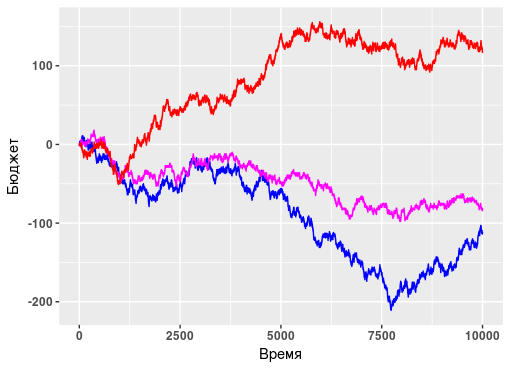
\includegraphics[scale=0.8]{parondo_game.png}
\end{center}




% \Closesolutionfile{solution_file}
% \input{solutions1}

\end{document}




